\documentclass[12pt,a4paper]{article}
\usepackage{header} % Use the provided header format
\usepackage[utf8]{inputenc}
\usepackage[T5]{fontenc}
\usepackage[vietnamese,english]{babel}

\begin{document}

\begin{center}
    \textbf{Digital Signal Processing \hfill HK261 \hfill CO2036}\\[2cm]
    
    \huge\textbf{DIGITAL SIGNAL PROCESSING LAB REPORT}\\[1cm]
    
    \large Âu Lê Quang Trí - Student ID: 2453300\\[0.5cm]
    \large Nguyễn Lê Khải Tú - Student ID: 2453384\\[1cm]
    
    \large \today\\[2cm]
\end{center}

\section*{Overview}
This report summarizes the results of the Digital Signal Processing laboratory exercises, specifically focusing on generating, manipulating, and analyzing discrete-time signals and systems using Scilab. The report covers Lab 1 and Lab 2.

\section{Introduction}
The laboratory exercises provide practical experience with continuous-time to discrete-time signal conversion, signal properties, and elementary discrete-time operations. By utilizing Scilab, theoretical concepts such as sampling, quantization, time-shifting, folding, and signal arithmetic are modeled and visualized to deepen our mathematical understanding.

\section{Objectives}
The objectives achieved upon completing these laboratory sessions include:
\begin{itemize}
    \item Utilizing Scilab for vector and matrix initializations.
    \item Understanding the sampling theorem and the quantization process (ADC procedure).
    \item Visualizing discrete signals via functions such as \texttt{plot2d3} and utilizing graph annotations.
    \item Implementing fundamental operations on discrete-time signals, including addition, multiplication, time-shifting, and time-reversal.
    \item Extracting the even and odd components of a given discrete-time sequence.
\end{itemize}

\section{Methodology}
The exercises were conducted on a Windows environment using the Scilab numerical computing software. Mathematical formulas from the time-domain representation of discrete signals were translated into Scilab scripts. Vectorized operations and padding techniques were applied where necessary to align discrete sequences prior to manipulation.

\section{Practical Contents}

\subsection{Lab 1}

\subsubsection*{Exercise 1.1}
\textbf{Question:} Using the operators in vector and matrix to do the following tasks:
\begin{itemize}
    \item Create a vector in the form of $(x_1+1, x_2+1, x_3+1, x_4+1)$ where $x_1, x_2, x_3, x_4$ are components of vector $x=1:4$.
    \item Create a vector in the form of $(x_1y_1, x_2y_2, x_3y_3, x_4y_4)$ where $x_1\dots x_4$ and $y_1\dots y_4$ are components of vector $x=1:4$ and vector $y=5:8$, respectively.
    \item Create a vector in the form of $(\sin(x_1), \sin(x_2), \dots, \sin(x_{10}))$ where $x$ is a vector of 10 values linearly chosen in the interval $[0, \pi]$.
\end{itemize}

\textbf{Explanation:} 
This exercise introduces element-wise vector operations in Scilab. 
\begin{itemize}
    \item For the first task, adding a scalar to a vector adds that scalar to every element identically: $x + 1 \Rightarrow [2, 3, 4, 5]$.
    \item The second task requires element-by-element multiplication (the Hadamard product). In Scilab, this is executed using the \texttt{.*} operator, multiplying elements at corresponding indices: $x .* y \Rightarrow [1\times 5, 2\times 6, 3\times 7, 4\times 8]$.
    \item The third task utilizes the \texttt{linspace(0, \%pi, 10)} function to generate an array of $N=10$ linearly spaced points. The \texttt{sin()} function is then mapped across the generated vector space.
\end{itemize}

\begin{figure}[H]
    \centering
    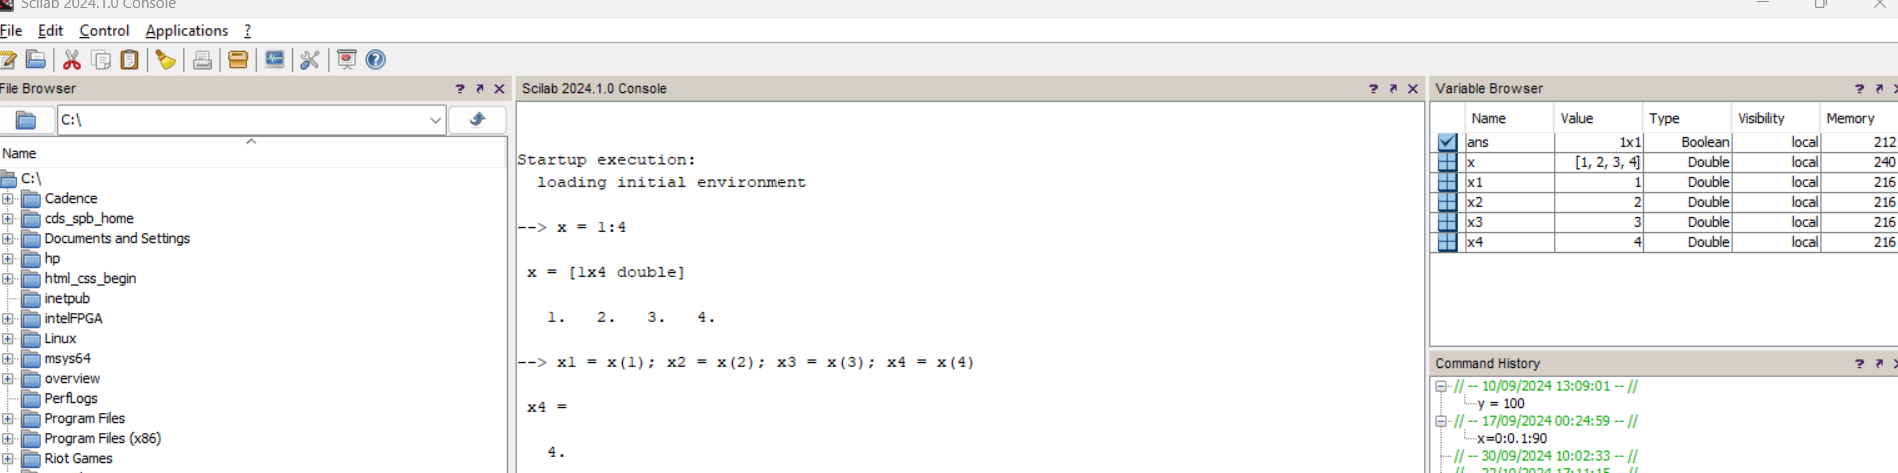
\includegraphics[width=0.7\textwidth]{extracted_images/Lab1_Ex1.1_1.png}
    \caption{Result of Ex 1.1 - Part 1}
\end{figure}

\begin{figure}[H]
    \centering
    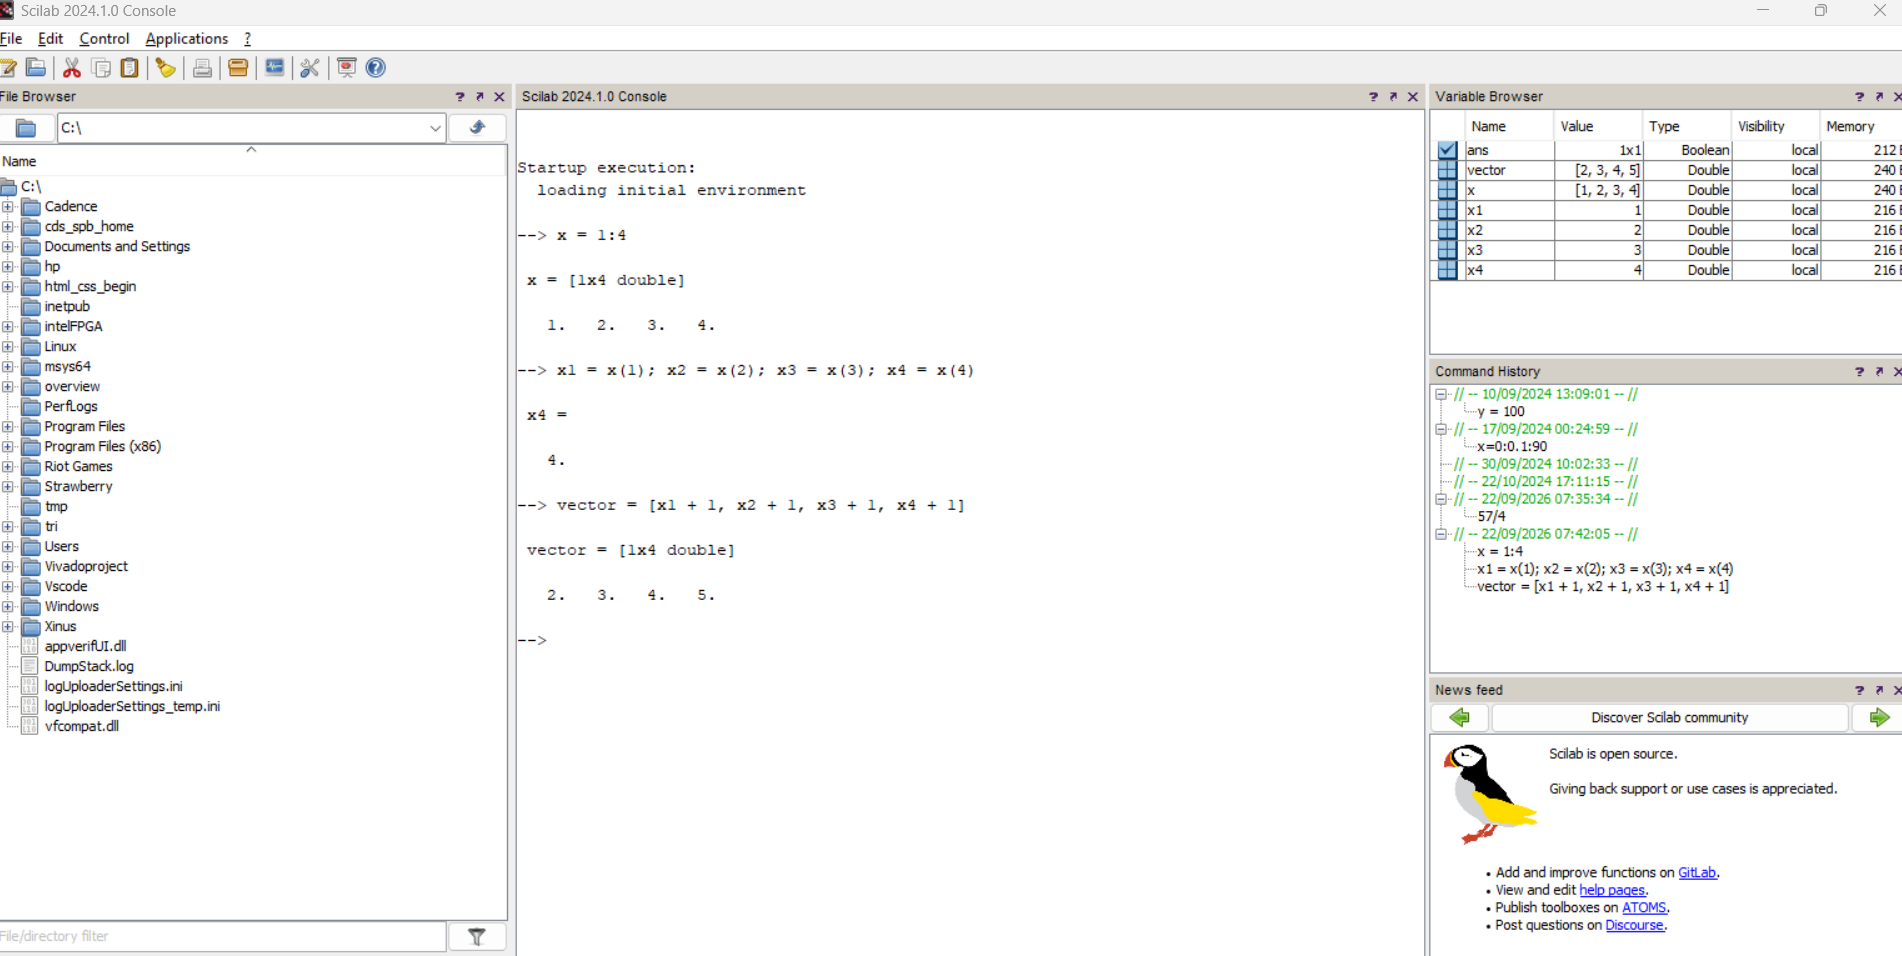
\includegraphics[width=0.7\textwidth]{extracted_images/Lab1_Ex1.1_2.png}
    \caption{Result of Ex 1.1 - Part 2}
\end{figure}

\subsubsection*{Exercise 1.2}
\textbf{Question:} Consider the analog signal $x_a(t) = 3\sin(100\pi t)$.
\begin{itemize}
    \item Use Scilab to draw $x_a(t)$ in 5 periods.
    \item Determine the discrete-time signal $x(n)$ of the signal $x_a(t)$ that is sampled with a sampling rate $F_s = 300$ samples/s.
    \item Determine the discrete-time signal $x(n)$ and determine its periodic property. If $x(n)$ is a periodic signal, determine the frequency and period of $x(n)$. Then, use Scilab to draw $x(n)$ in 5 periods.
    \item Determine the quantized signal $x_q(n)$ if $\Delta = 0.1$ using the truncated method. Then, draw $x_q(n)$ in 5 periods. All figures must be displayed in a single window.
\end{itemize}

\textbf{Explanation:}
Given $x_a(t) = 3\sin(100\pi t)$, the analog frequency is $F_0 = 50$ Hz. By applying the sampling theorem with $F_s = 300$ Hz, the sampling interval is $T_s = 1/F_s$. Substituting $t = nT_s$:
\begin{equation}
    x(n) = x_a(nT_s) = 3\sin\left(100\pi \frac{n}{300}\right) = 3\sin\left(\frac{\pi}{3} n\right)
\end{equation}
A discrete sinusoid is periodic if its digital frequency $f = \frac{F_0}{F_s} = \frac{50}{300} = \frac{1}{6}$ is a rational number. Because $f = \frac{1}{6}$, $x(n)$ is periodic. The fundamental period is determined by $N = \frac{K}{f}$ where $K$ is the smallest integer yielding an integer $N$. Thus, for $K=1$, the discrete period is $N = 6$ samples.

For quantization, we apply a truncation method with step size $\Delta = 0.1$. The truncated value $x_q(n)$ is obtained via the floor operation after normalizing by $\Delta$:
\begin{equation}
    x_q(n) = \Delta \lfloor \frac{x(n)}{\Delta} \rfloor = 0.1 \lfloor 10 \cdot x(n) \rfloor
\end{equation}

\begin{figure}[H]
    \centering
    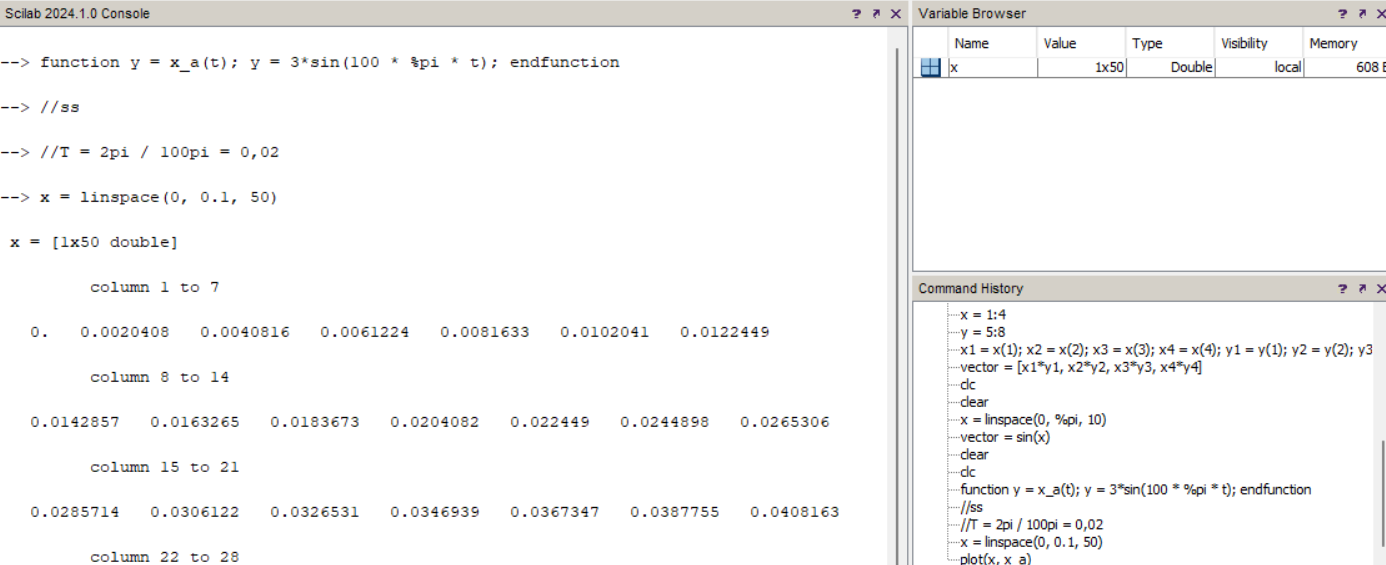
\includegraphics[width=0.7\textwidth]{extracted_images/Lab1_Ex1.2_1.png}
    \caption{Result of Ex 1.2 - Analog and Discrete Signal}
\end{figure}

\begin{figure}[H]
    \centering
    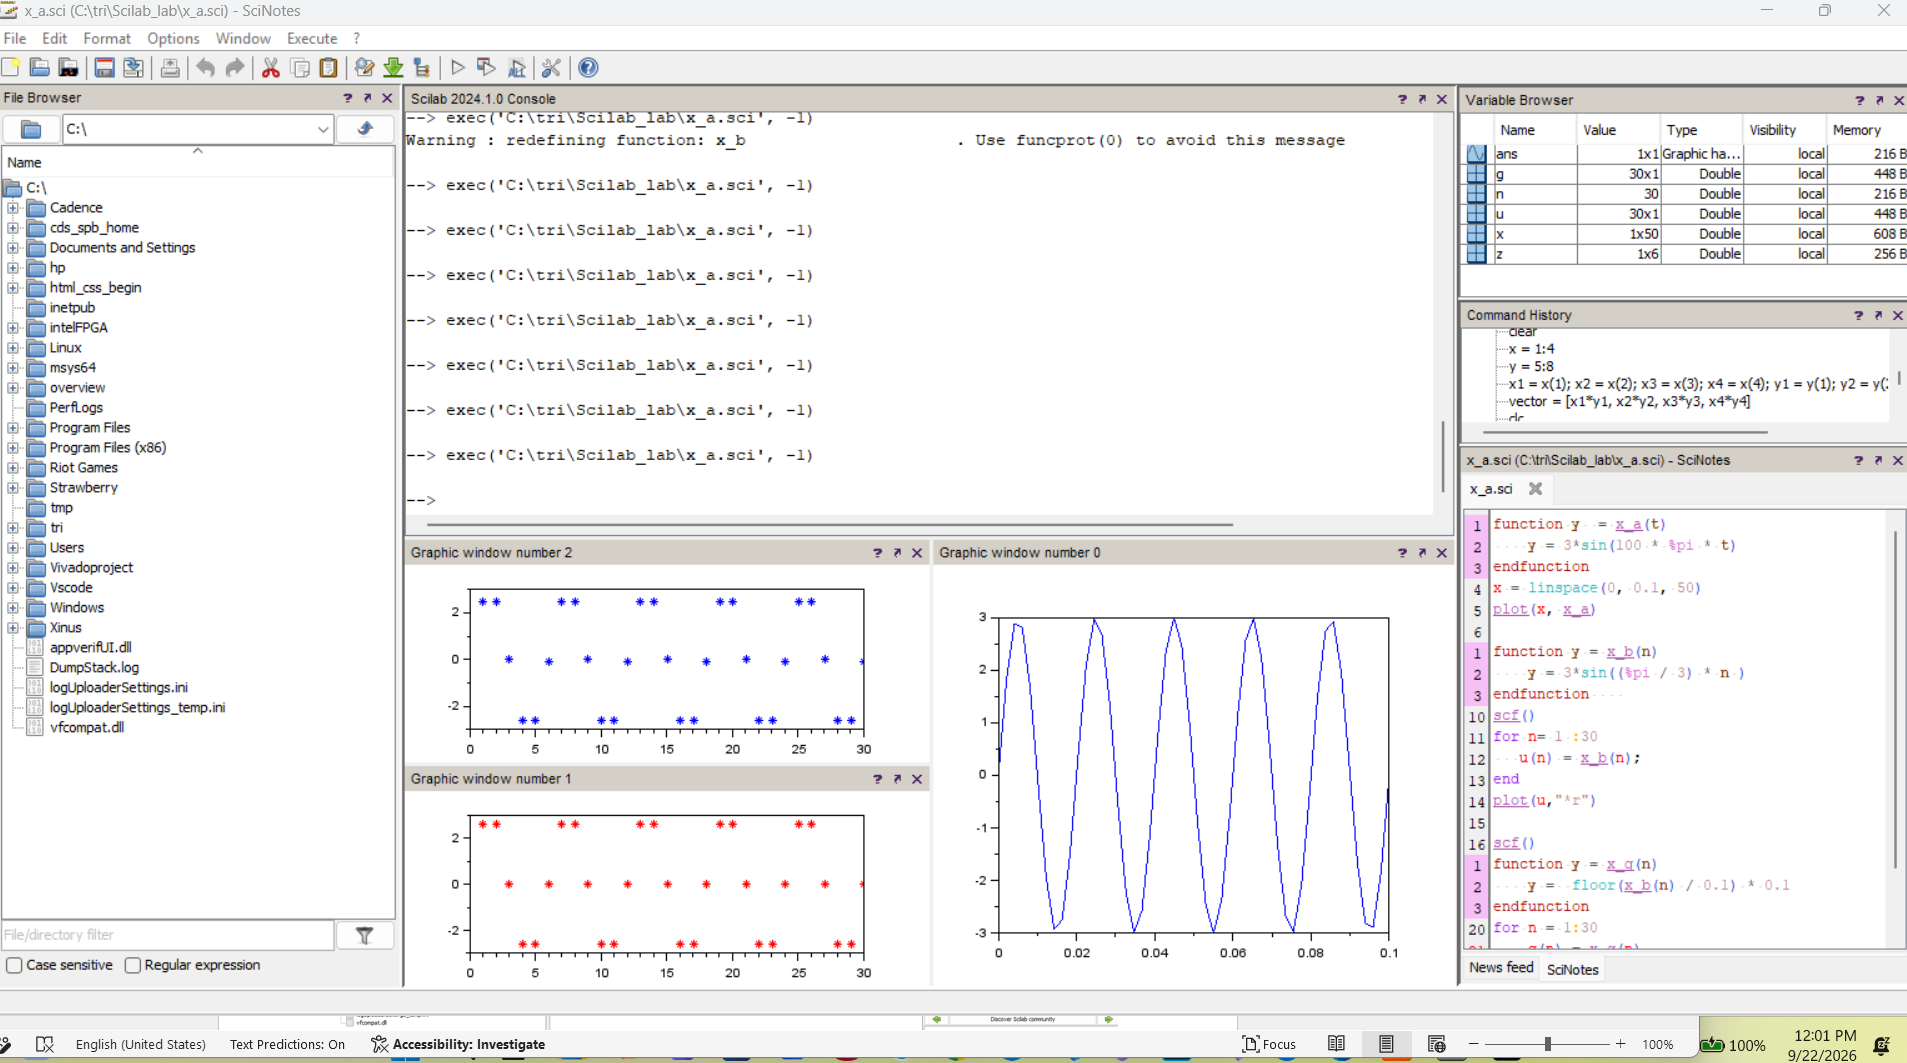
\includegraphics[width=0.7\textwidth]{extracted_images/Lab1_Ex1.2_2.png}
    \caption{Result of Ex 1.2 - Quantized Signal and Errors}
\end{figure}

\subsection{Lab 2}

\subsubsection*{Exercise 1: Investigate Basic Functions}
\textbf{Question:} Let's investigate the following functions on Scilab and briefly report their functionalities and how to use it: \texttt{plot2d3, min, max, subplot, title, xlabel, ylabel, bool2s, deff}.

\textbf{Explanation:}
This exercise evaluates fundamental plotting and computational functions:
\begin{itemize}
    \item \texttt{plot2d3(x, y)}: Plots vertical lines (stems) representing discrete-time samples. It is strictly used for discrete signals to highlight values at integer indices.
    \item \texttt{max()} and \texttt{min()}: Calculates the maximum/minimum elements in a matrix or vector array, highly useful for determining normalization constants or quantization step limits.
    \item \texttt{subplot(m, n, p)}: Divides the graphic window into an $m \times n$ matrix of sub-windows, selecting the $p^{th}$ window for the active plot.
    \item \texttt{title()}, \texttt{xlabel()}, \texttt{ylabel()}: These functions add textual annotations to the graph. \texttt{title()} sets the main heading, while \texttt{xlabel()} and \texttt{ylabel()} label the respective axes, which is crucial for identifying discrete components properly.
    \item \texttt{bool2s()}: Converts a boolean array containing \%T and \%F into a numerical array of 1s and 0s. This is mathematically equivalent to the Heaviside step function evaluating a logic condition.
    \item \texttt{deff()}: Defines inline custom functions on the fly, similar to lambda expressions. Syntax: \texttt{deff("[y] = f(x)", "y = ...")}.
\end{itemize}

\begin{figure}[H]
    \centering
    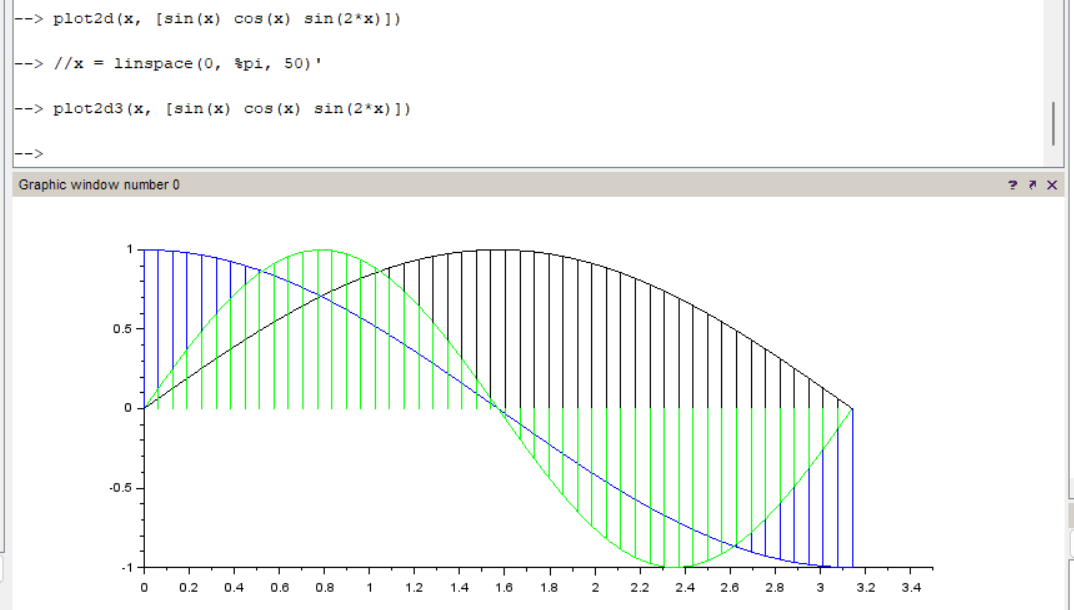
\includegraphics[width=0.45\textwidth]{extracted_images/Lab2_Ex1_plot2d3_2.png}
    \caption{plot2d3 Usage}
\end{figure}
\begin{figure}[H]
    \centering
    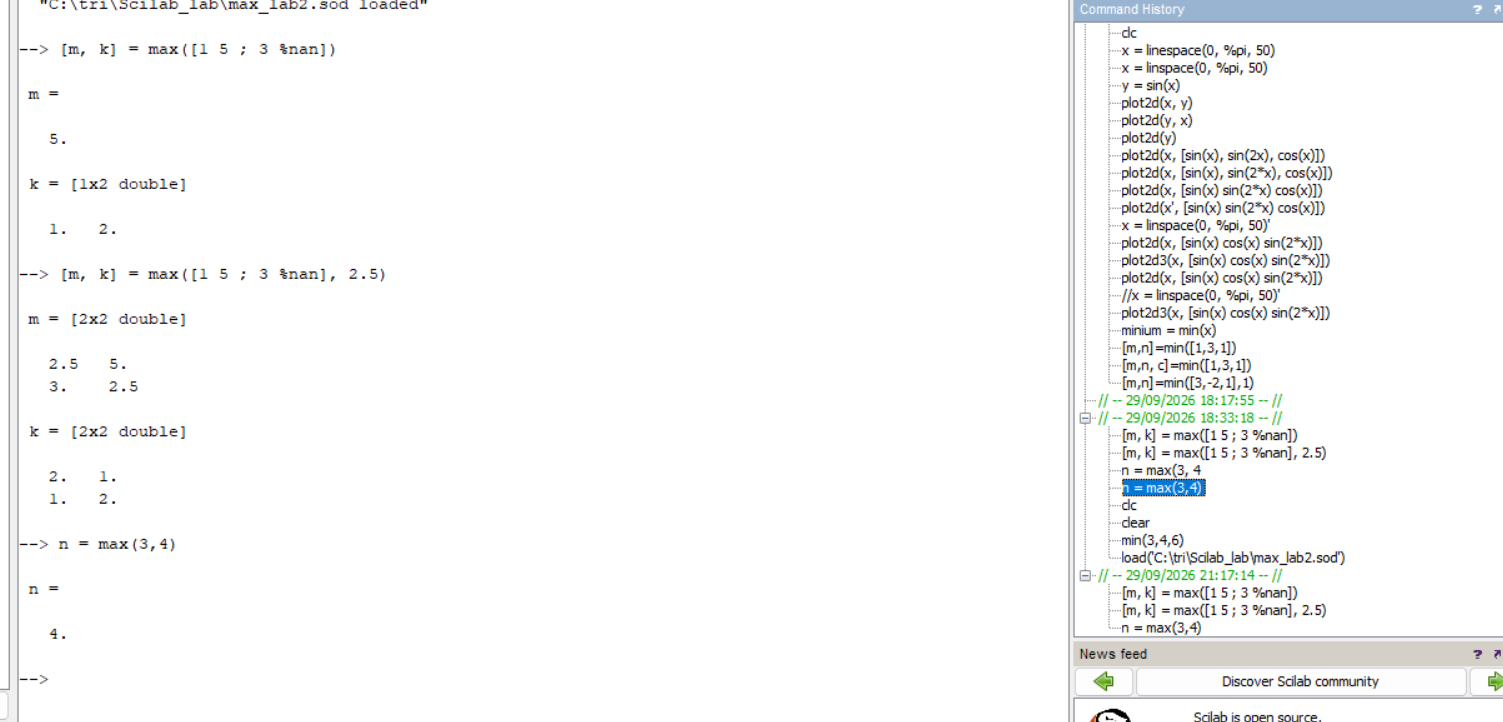
\includegraphics[width=0.45\textwidth]{extracted_images/Lab2_Ex1_max.png}
    \caption{max() Usage}
\end{figure}
\begin{figure}[H]
    \centering
    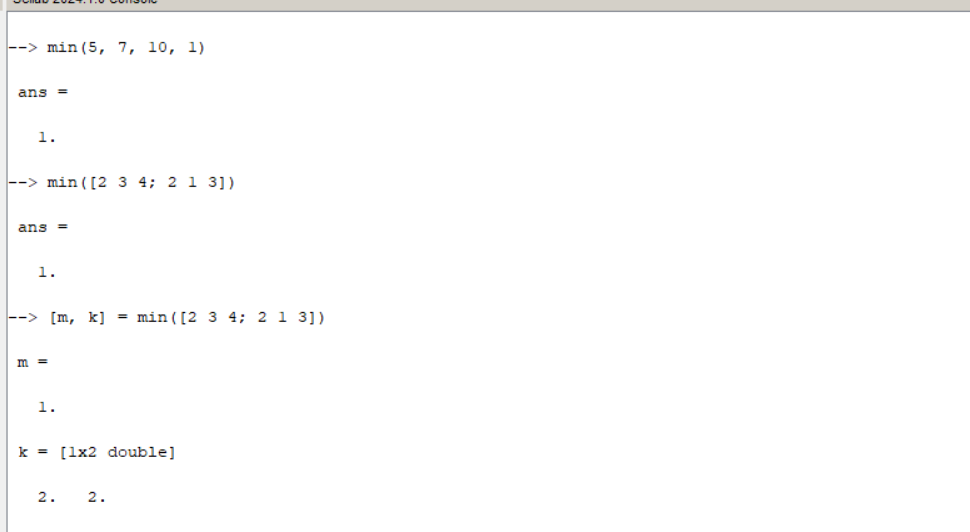
\includegraphics[width=0.45\textwidth]{extracted_images/Lab2_Ex1_min_1.png}
    \caption{min() Usage}
\end{figure}
\begin{figure}[H]
    \centering
    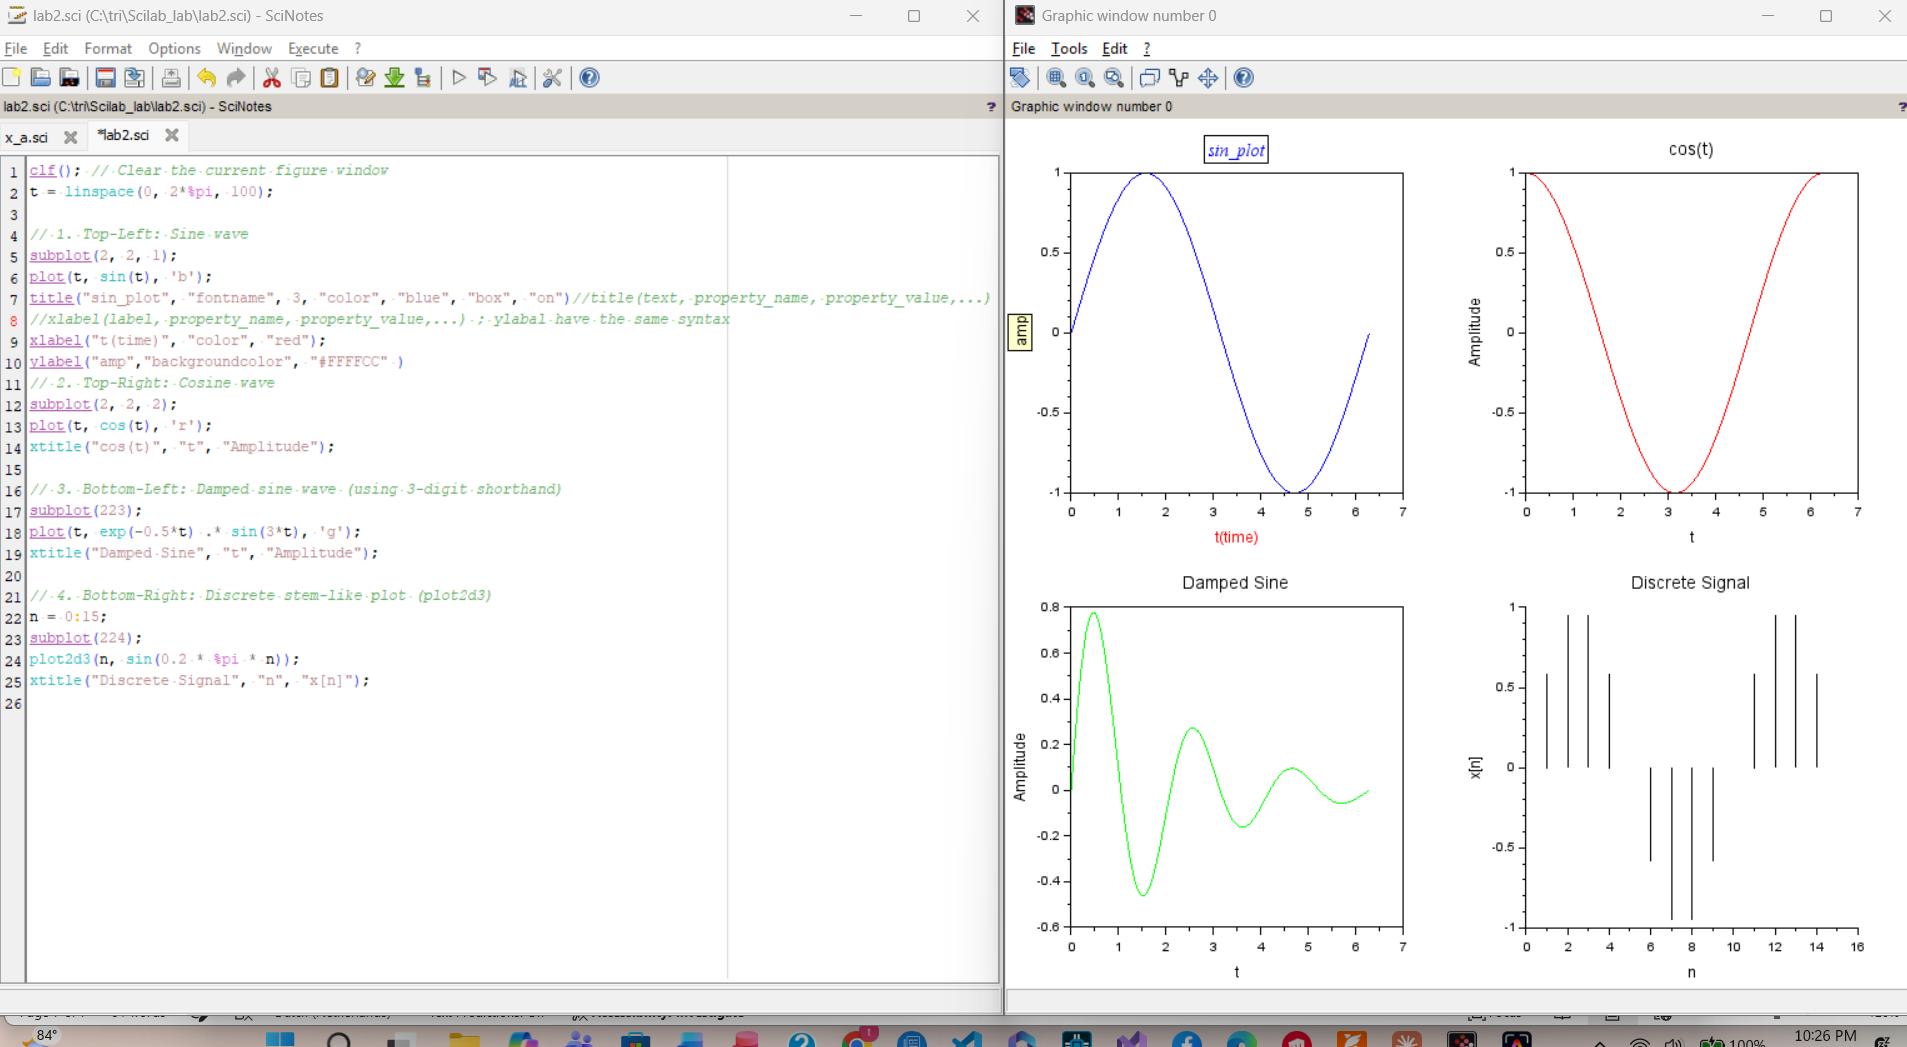
\includegraphics[width=0.45\textwidth]{extracted_images/Lab2_Ex1_subplot_1.png}
    \caption{subplot() + title() + xlabel() + ylabel() Usage}
\end{figure}
\begin{figure}[H]
    \centering
    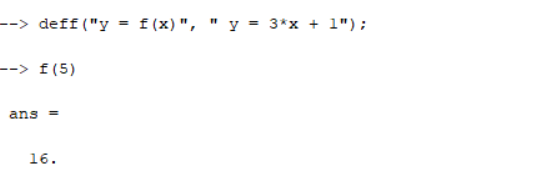
\includegraphics[width=0.6\textwidth]{extracted_images/Lab2_Ex1_deff.png}
    \caption{deff Usage}
\end{figure}

\subsubsection*{Exercise 2 \& Exercise 3}
\textbf{Question:} Try the following scripts on Scilab and report your understanding after observing the output.
\begin{itemize}
    \item \texttt{n = -5:5; msignal = bool2s(n >= 0); plot2d3(n, msignal)}
    \item \texttt{n = -5:5; msignal = bool2s(n == 0); plot2d3(n, msignal)}
\end{itemize}

\textbf{Explanation:}
\begin{itemize}
    \item \textbf{Exercise 2:} The logical condition \texttt{n >= 0} evaluates to True for $n \ge 0$ and False otherwise. \texttt{bool2s} transforms these booleans into numeric 1s and 0s. The output precisely replicates the mathematical definition of a \textbf{unit step sequence} $u(n)$:
    \begin{equation}
        u(n) = \begin{cases} 1, & n \ge 0 \\ 0, & n < 0 \end{cases}
    \end{equation}
    \item \textbf{Exercise 3:} The equality \texttt{n == 0} is true only at the origin point $n = 0$. Consequently, applying \texttt{bool2s} creates a sequence that represents the \textbf{unit sample sequence (discrete Dirac delta function)} $\delta(n)$:
    \begin{equation}
        \delta(n) = \begin{cases} 1, & n = 0 \\ 0, & n \neq 0 \end{cases}
    \end{equation}
\end{itemize}

\begin{figure}[H]
    \centering
    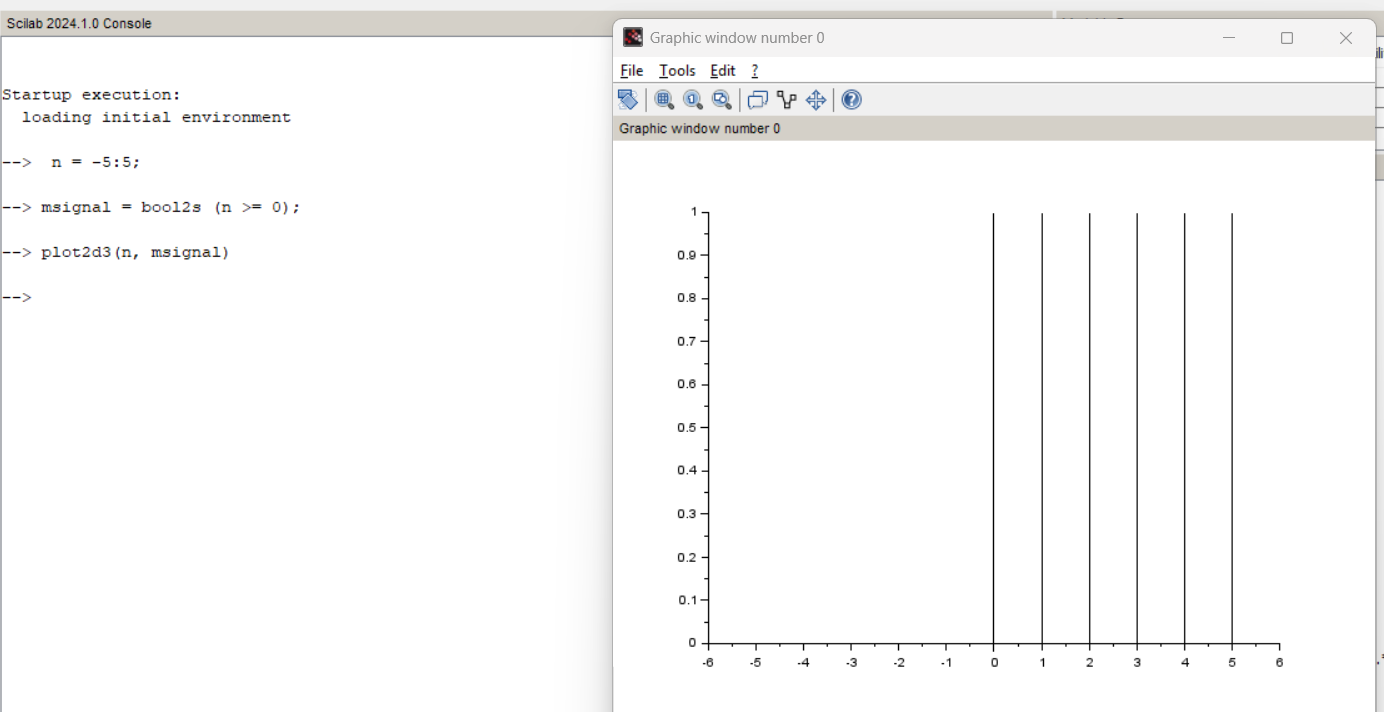
\includegraphics[width=0.6\textwidth]{extracted_images/Lab2_Ex2.png}
    \caption{Result of Ex 2 - Unit Step Sequence $u(n)$}
\end{figure}
\begin{figure}[H]
    \centering
    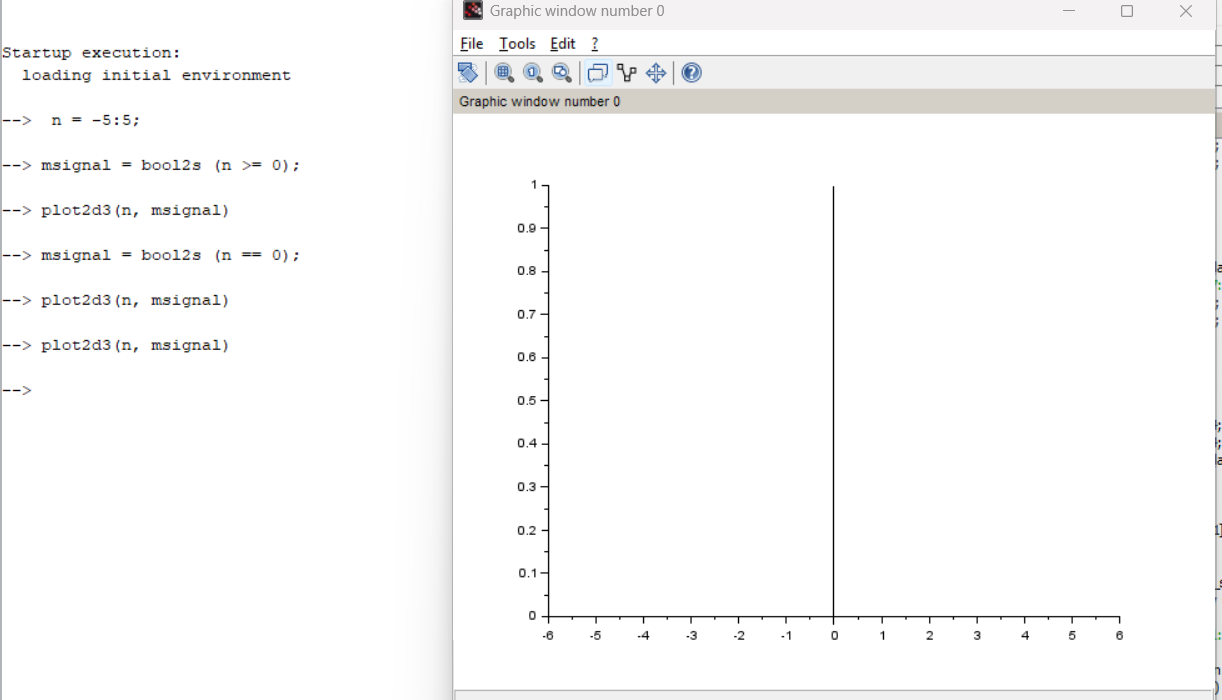
\includegraphics[width=0.6\textwidth]{extracted_images/Lab2_Ex3.png}
    \caption{Result of Ex 3 - Unit Sample Sequence $\delta(n)$}
\end{figure}

\subsubsection*{Exercise 4: Unit Ramp Signal}
\textbf{Question:} Use Scilab to draw the unit ramp signal $u_r(n)$ for $n=-5:5$.

\textbf{Explanation:} The discrete unit ramp signal is mathematically defined as the integral of the unit step function, or more precisely:
\begin{equation}
    u_r(n) = n \cdot u(n) = \begin{cases} n, & n \ge 0 \\ 0, & n < 0 \end{cases}
\end{equation}
In Scilab, this is implemented natively by executing an element-wise product between the index space array $n$ and the previously defined unit step array.

\begin{figure}[H]
    \centering
    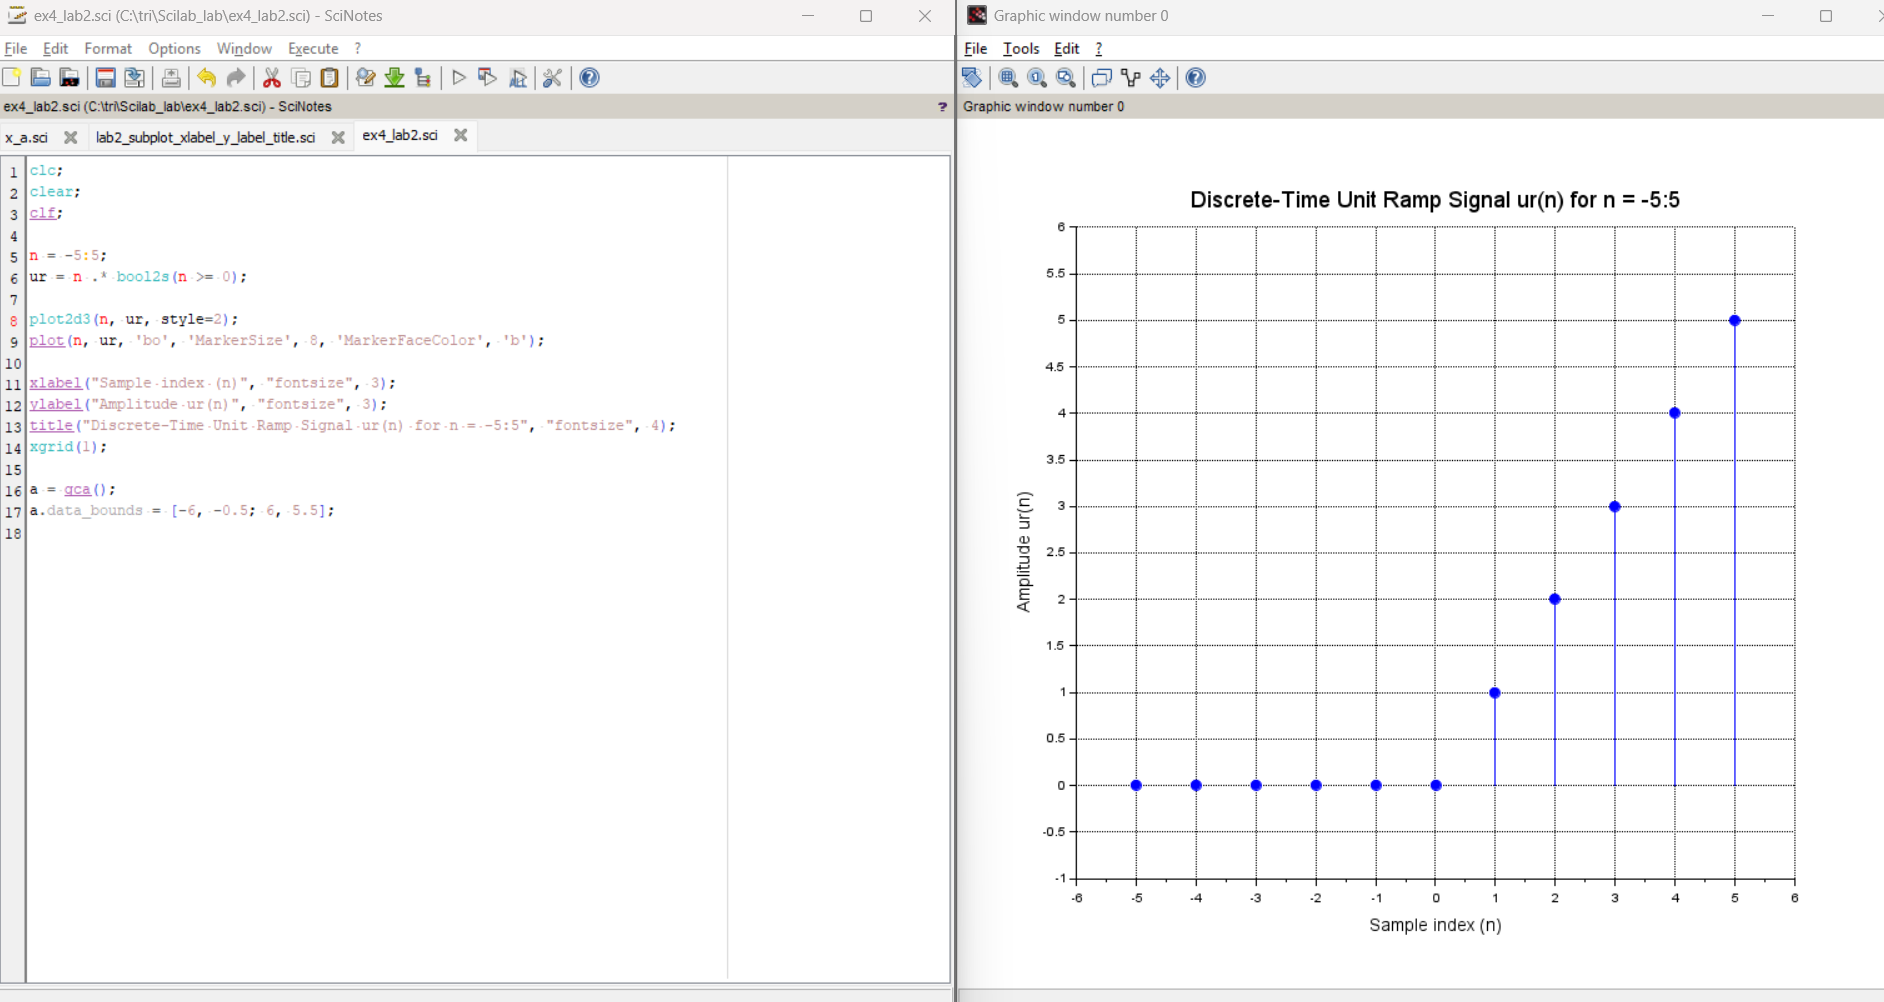
\includegraphics[width=0.6\textwidth]{extracted_images/Lab2_Ex4.png}
    \caption{Result of Ex 4 - Unit Ramp Signal}
\end{figure}

\subsubsection*{Exercise 5: Even and Odd Components}
\textbf{Question:} Given a discrete-time signal $x(n)=\{1, 3\uparrow, -2\}$. Use Scilab to draw the signal $x(n)$, the odd signal component $x_o(n)$, and the even signal component $x_e(n)$.

\textbf{Explanation:} 
The arrow signifies the origin index $n=0$. The sequence is thus explicitly indexed as $x(-1)=1, x(0)=3, x(1)=-2$. 
According to signal properties, any arbitrary sequence can be perfectly decomposed into an even-symmetric component $x_e(n)$ and an odd-symmetric component $x_o(n)$. 
We first evaluate the folded (time-reversed) sequence $x(-n)$. Using the decomposition formula:
\begin{equation}
    x_e(n) = \frac{x(n) + x(-n)}{2}, \quad x_o(n) = \frac{x(n) - x(-n)}{2}
\end{equation}
Calculations yield $x_e(-1) = -0.5, x_e(0) = 3, x_e(1) = -0.5$, and correspondingly $x_o(-1) = 1.5, x_o(0) = 0, x_o(1) = -1.5$. Scilab strictly mirrors these mathematical operations linearly. Therefore, the resulting sequences are:
\begin{equation}
    x_e(n) = \{-0.5, 3\uparrow, -0.5\}, \quad x_o(n) = \{1.5, 0\uparrow, -1.5\}
\end{equation}

\begin{figure}[H]
    \centering
    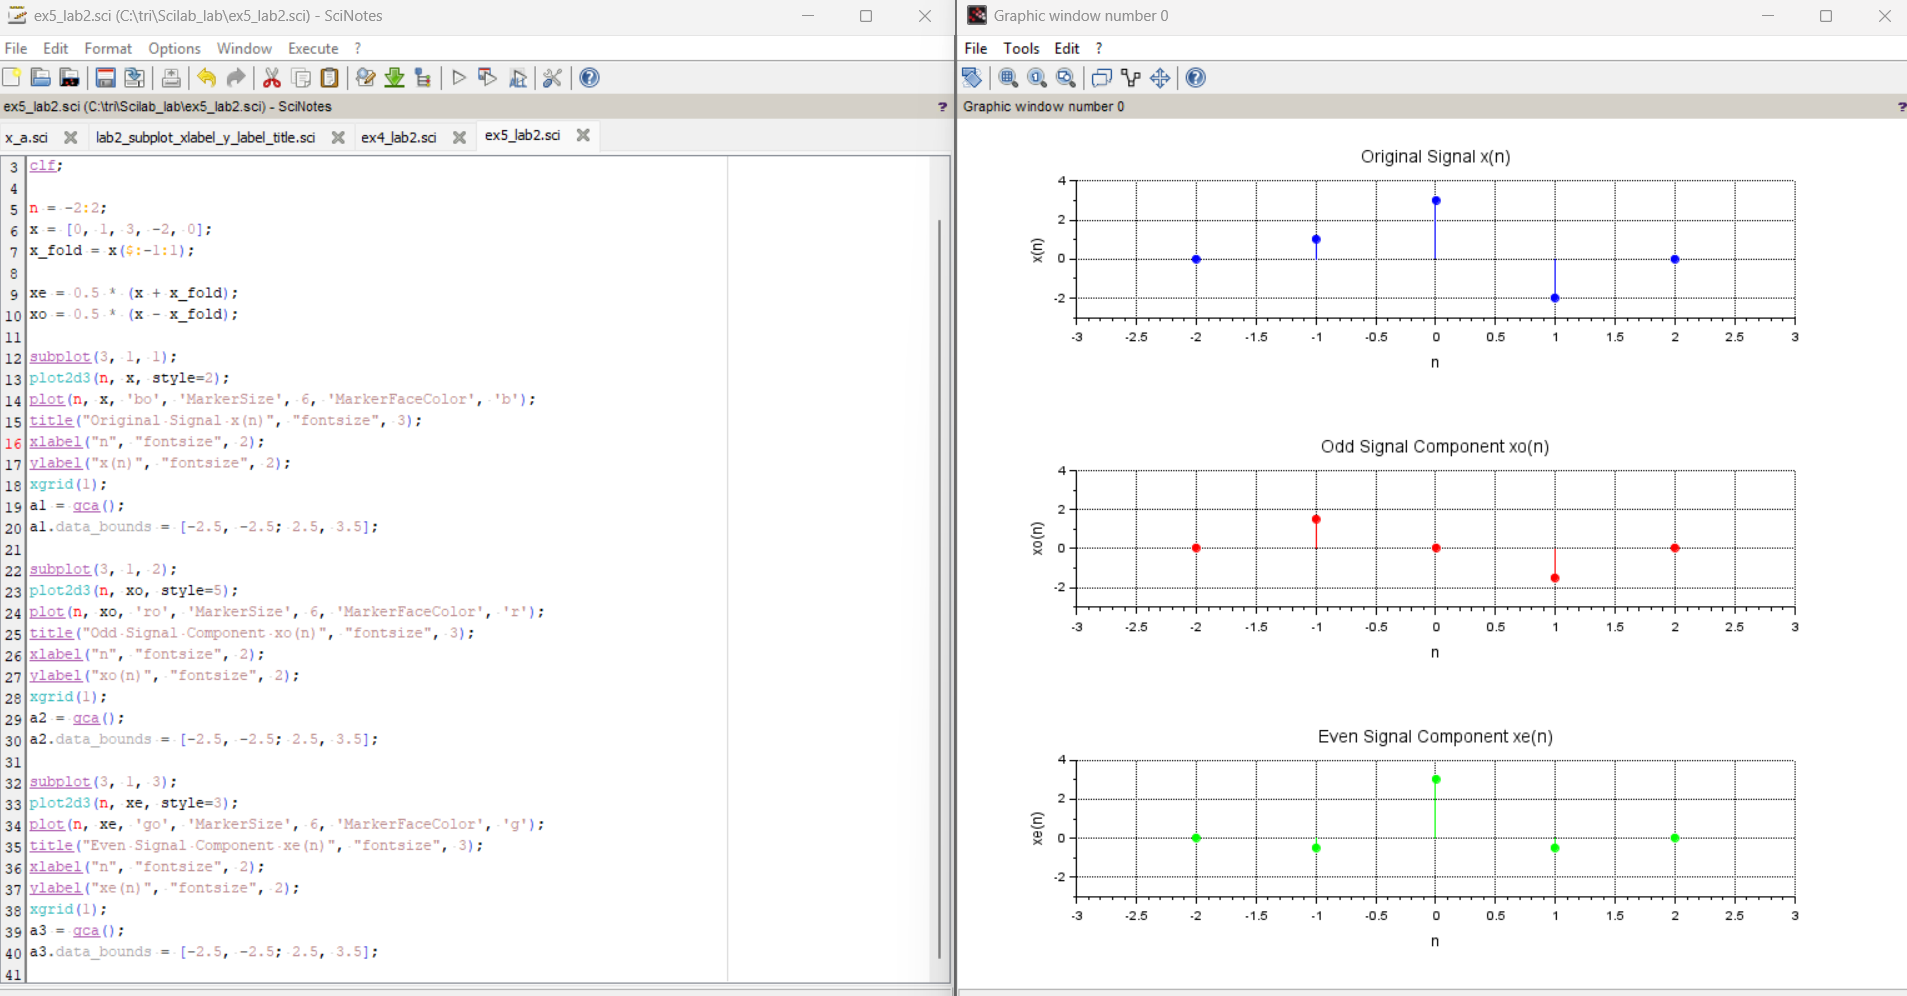
\includegraphics[width=0.7\textwidth]{extracted_images/Lab2_Ex5.png}
    \caption{Result of Ex 5 - Even and Odd Decomposition}
\end{figure}

\subsubsection*{Exercise 6 \& 7: Addition and Multiplication of Signals}
\textbf{Question:} 
\begin{itemize}
    \item \textbf{Exercise 6:} Given two discrete-time signals $x_1(n)=\{0\uparrow, 1, 3, -2\}$ and $x_2(n)=\{0, 1\uparrow, 2, 3\}$. Determine $y(n) = x_1(n) + x_2(n)$.
    \item \textbf{Exercise 7:} Given the same signals, determine $y(n) = x_1(n) \cdot x_2(n)$.
\end{itemize}

\textbf{Explanation:}
Because the two sequences span different bounded domain intervals ($x_1(n)$ spans $[0, 3]$ and $x_2(n)$ spans $[-1, 2]$), they cannot be directly operated on using primitive arrays.
To implement a rigorous sample-by-sample operation, we determine the union of both index domains: $[\min(n_{1_{min}}, n_{2_{min}}), \max(n_{1_{max}}, n_{2_{max}})] = [-1, 3]$. Both vectors are then symmetrically zero-padded to conform to this unified domain grid.
Once the sequences structurally align relative to the time origin $n=0$:
\begin{equation}
    y_{add}(n) = x_1(n) + x_2(n) = \{0, 1\uparrow, 3, 6, -2\}
\end{equation}
\begin{equation}
    y_{mult}(n) = x_1(n) \cdot x_2(n) = \{0, 0\uparrow, 2, 9, 0\} \text{ or simply } \{0\uparrow, 2, 9\}
\end{equation}

\begin{figure}[H]
    \centering
    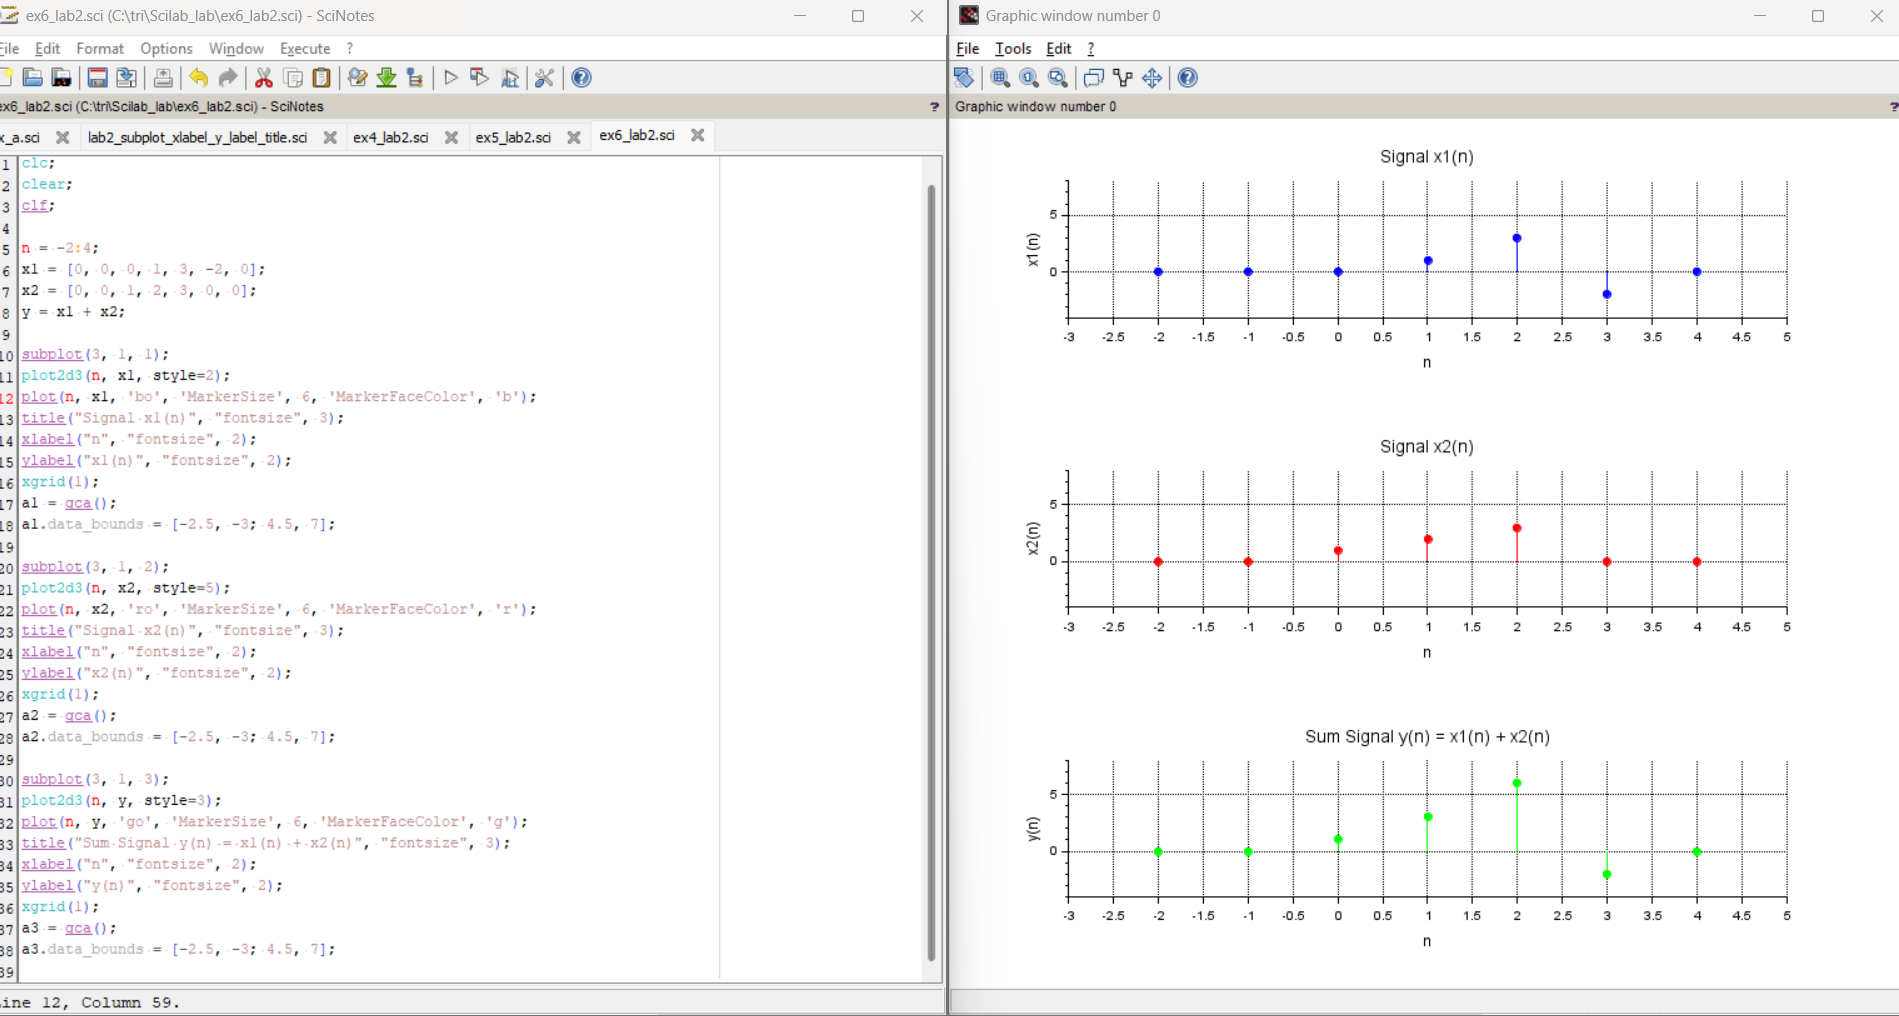
\includegraphics[width=0.7\textwidth]{extracted_images/Lab2_Ex6.png}
    \caption{Result of Ex 6 - Addition of Signals}
\end{figure}
\begin{figure}[H]
    \centering
    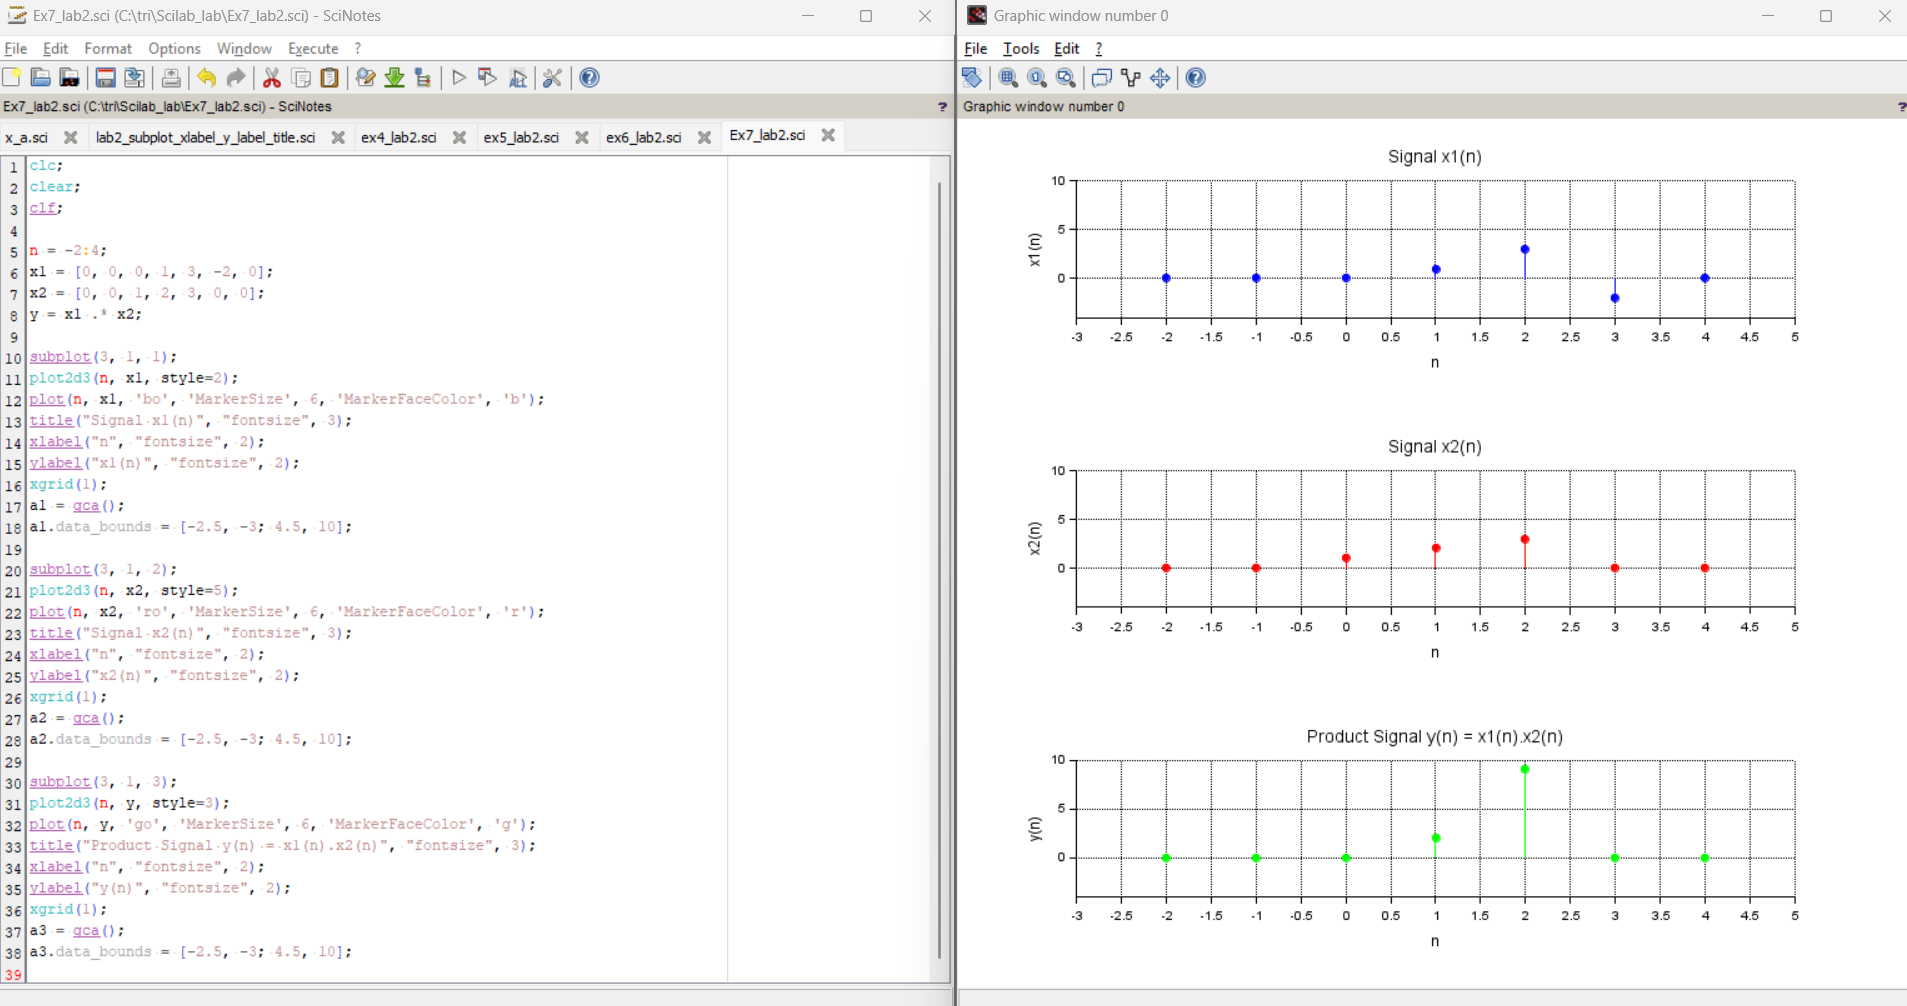
\includegraphics[width=0.7\textwidth]{extracted_images/Lab2_Ex7.png}
    \caption{Result of Ex 7 - Multiplication of Signals}
\end{figure}

\subsubsection*{Exercise 8: Signal Manipulations}
\textbf{Question:} Given a discrete-time signal $x(n)=\{1, -2, 3\uparrow, 6\}$. Determine the following signals and draw both original and manipulated signals:
1. $y_1(n) = x(-n)$
2. $y_2(n) = x(n+3)$
3. $y_3(n) = 2x(-n-2)$

\textbf{Explanation:}
For $x(n)$, the origin translates to $x(-2)=1, x(-1)=-2, x(0)=3, x(1)=6$. We systematically apply independent operations on the sequence index variables:
\begin{enumerate}
    \item \textbf{Folding (Time-Reversal):} $y_1(n) = x(-n)$. Every index evaluates to its symmetrical negative counterpart. Resulting indices: $[-1, 2]$. 
    \begin{equation}y_1(n) = \{6, 3\uparrow, -2, 1\}\end{equation}
    \item \textbf{Advance (Time-Shift):} $y_2(n) = x(n+3)$. The addition inside the argument denotes an advancement. The whole sequence is shifted to the left along the time axis by 3 sample units.
    \begin{equation}y_2(n) = \{1, -2, 3, 6, 0, 0\uparrow\}\end{equation}
    \item \textbf{Composite Operations:} $y_3(n) = 2x(-(n+2))$. To evaluate this correctly: first perform folding to get $x(-n)$, then shift left by 2 to get $x(-(n+2))$, and finally apply an amplitude scaling factor of $2$.
    \begin{equation}y_3(n) = \{12, 6, -4, 2\uparrow\}\end{equation}
\end{enumerate}

\begin{figure}[H]
    \centering
    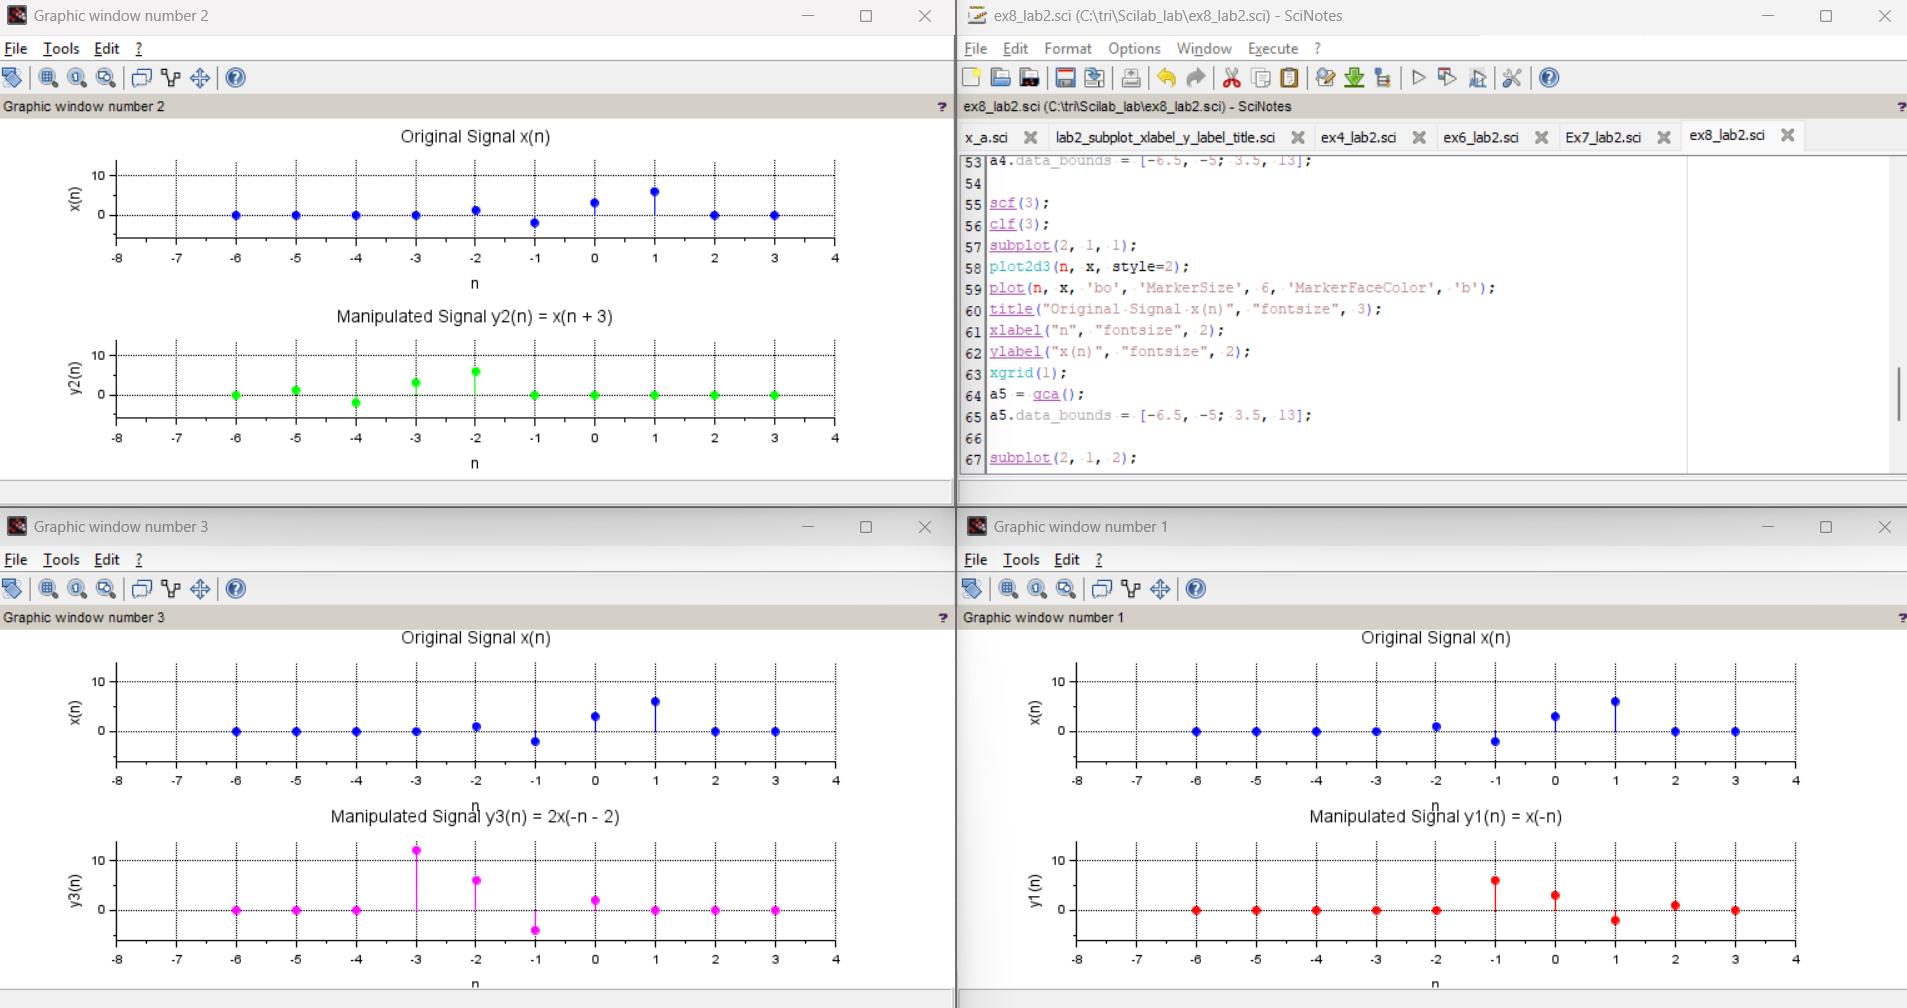
\includegraphics[width=0.7\textwidth]{extracted_images/Lab2_Ex8.png}
    \caption{Result of Ex 8 - Signal Manipulations}
\end{figure}

\subsubsection*{Additional exercise 1.1}
\noindent
Classify the following signals according to whether they are (1) one- or multi-dimensional; (2) single or multichannel, (3) continuous time or discrete time, and (4) analog or digital (in amplitude). Give a brief explanation.

\begin{enumerate}[label=\textbf{(\alph*)}, leftmargin=*]
    \item Closing prices of utility stocks on the New York Stock Exchange.
    \item A color movie.
    \item Position of the steering wheel of a car in motion relative to car's reference frame.
    \item Position of the steering wheel of a car in motion relative to ground reference frame.
    \item Weight and height measurements of a child taken every month.
\end{enumerate}

\noindent\textbf{Answer:}
\begin{enumerate}[label=\textbf{(\alph*)}, leftmargin=*]
    \item (1) One dimensional because closing prices are functions of time.\\
    (2) Multichannel because the signal is a vector of prices.\\
    (3) Discrete-time because closing prices are defined only at a specific instance of time.\\
    (4) Digital because prices are money, which is discrete-valued.
    \item (1) Multidimensional because light characteristics at each point is a function of 2-D coordinates and time.\\
    (2) "Movie" in this context refers to traditional film, which is single channel.\\
    (3) Continuous-time because light characteristics are defined at every point in time as the film rolls.\\
    (4) Analog because light has a continuous physical properties.
    \item (1) One dimensional because position is a function of time.\\
    (2) "Position" in this context refers to the angular rotation of the steering wheel, which means single channel.\\
    (3) Continuous-time because position is defined at every point in time.\\
    (4) Analog because angular position is a continuous physical quantity.
    \item (1) One dimensional, (2) single channel, (3) continuous-time, (4) analog.
    \item (1) One dimensional because height and weight are functions of time.\\
    (2) Multichannel because the signal consists of height and weight.\\
    (3) Discrete-time because height and weight are only measured monthly.\\
    (4) Digital because measured height and weight are discrete valued while physical height and weight are analog valued.
\end{enumerate}

\subsubsection*{Additional exercise 1.3}
\noindent
Determine whether or not each of the following signals is periodic. In case a signal is periodic, specify its fundamental period.

\begin{enumerate}[label=\textbf{(\alph*)}, leftmargin=*]
    \item $x_a(t) = 3 \cos(5t + \pi/6)$
    \item $x(n) = 3 \cos(5n + \pi/6)$
    \item $x(n) = 2 \exp[j(n/6 - \pi)]$
    \item $x(n) = \cos(n/8) \cos(\pi n/8)$
    \item $x(n) = \cos(\pi n/2) - \sin(\pi n/8) + 3 \cos(\pi n/4 + \pi/3)$
\end{enumerate}

\noindent\textbf{Answer:}
\begin{enumerate}[label=\textbf{(\alph*)}, leftmargin=*]
    \item $T_p=\frac{1}{F}=\frac{2\pi}{5}$. We have
    \begin{align*}
        x_a(t+T_p)&=3cos(2\pi\frac{5}{2\pi}t+2\pi+\frac{\pi}{6})\\
        &=3cos(5t+\frac{\pi}{6})\\
        &=x_a(t)\\
        &\Rightarrow Periodic
    \end{align*}
    \item $x(n) = 3 \cos(5n + \pi/6)=3\cos(2\pi\frac{5}{2\pi}n+\pi/6)$. $f=\frac{5}{2\pi}$ is not rational, therefore not periodic.
    \item $x(n) = 2 \exp[j(n/6 - \pi)]=2e^{j(2\pi\frac{1}{12\pi}n-\pi)}$. $f=\frac{1}{12\pi}$ is not rational, therefore not periodic.
    \item $\cos(n/8)$ is nonperiodic, $\cos(\pi n/8)$ is periodic, their product is nonperiodic.
    \item $x(n) = \cos(\pi n/2) - \sin(\pi n/8) + 3 \cos(\pi n/4 + \pi/3) = \cos(2\pi \frac{1}{4}n) - \sin(2\pi\frac{1}{16} n) + 3 \cos(2\pi\frac{1}{8}n + \pi/3)$.
    $\cos(2\pi \frac{1}{4}n)$ is periodic with $N=4$, $ \sin(2\pi\frac{1}{16} n) $ is periodic $N=16$, $3 \cos(2\pi\frac{1}{8}n + \pi/3)$ is periodic with $N=8$.
    Therefore $x(n)$ is periodic with $N=LCM(4,16,8)=16$.
\end{enumerate}

\subsubsection*{Additional exercise 1.6}
\noindent
A continuous-time sinusoid $x_a(t)$ with fundamental period $T_p = 1/F_0$ is sampled at a rate $F_s = 1/T$ to produce a discrete-time sinusoid $x(n) = x_a(nT)$.

\begin{enumerate}[label=\textbf{(\alph*)}, leftmargin=*]
    \item Show that $x(n)$ is periodic if $T/T_p = k/N$ (i.e., $T/T_p$ is a rational number).
    \item If $x(n)$ is periodic, what is its fundamental period $T_p$ in seconds?
    \item Explain the statement: $x(n)$ is periodic if its fundamental period $T_p$, in seconds, is equal to an integer number of periods of $x_a(t)$.
\end{enumerate}

\noindent\textbf{Answer:}
\begin{enumerate}[label=\textbf{(\alph*)}, leftmargin=*]
    \item We have
    \[\frac{T}{T_p}=\frac{1/F_s}{1/F_0}=\frac{F_0}{F_s}\]
    and
    \[x(n)=A\cos(2\pi\frac{F_0}{F_s}n+\theta)\]
    Thus, $x(n)$ is periodic if $T/T_p$ is rational.
    \item When $x(n)$ is periodic, we have $f_0 = F_0/F_s = k/N \rightarrow N = k/f_0$.
    Suppose the fundamental period of $x(n)$ is $T_d=NT$, we have $T_d = (\frac{k}{f_0})T = k(\frac{T_p}{T})T = kT_p$.
    Thus it takes $kT_p$ seconds to make 1 period $T_d$ of $x(n)$.
    \item $T_d = kT_p \Leftrightarrow NT = kT_p \Rightarrow f = k/N = T/T_p \Rightarrow \text{f is rational}\Rightarrow \text{$x(n)$ is periodic}$.
\end{enumerate}
\subsubsection*{Additional exercise 1.7}
\noindent
An analog signal contains frequencies up to $10\text{ kHz}$.

\begin{enumerate}[label=\textbf{(\alph*)}, leftmargin=*]
    \item What range of sampling frequencies allows exact reconstruction of this signal from its samples?
    \item Suppose that we sample this signal with a sampling frequency $F_s = 8\text{ kHz}$. Examine what happens to the frequency $F_1 = 5\text{ kHz}$.
    \item Repeat part (b) for a frequency $F_2 = 9\text{ kHz}$.
\end{enumerate}

\noindent\textbf{Answer:}
\begin{enumerate}[label=\textbf{(\alph*)}, leftmargin=*]
    \item $F_s\geq 2F_{max} = 20\: kHz$.
    \item With $F_s = 8\: kHz$, only signals in the range $-F_s/2\leq F \leq F_s/2$ can be reconstructed exactly.
    The frequency $F_1=5\: kHz$ is folded with the folding frequency $F_s/2 = 4\: kHz$ $F_1'=F_1-kF_s = 5000 - k8000 = -3000\: Hz\:(\text{with $k=1$})$.
    \item $F_2 = 9\: kHz$ gets folded to $F_2' = F_2 - kF_s=9000-k8000= 1000\: Hz\: (\text{with $k=1$})$.
\end{enumerate}

\subsubsection*{Additional exercise 1.9}
\noindent
An analog signal $x_a(t) = \sin(480\pi t) + 3 \sin(720\pi t)$ is sampled 600 times per second.

\begin{enumerate}[label=\textbf{(\alph*)}, leftmargin=*]
    \item Determine the Nyquist sampling rate for $x_a(t)$.
    \item Determine the folding frequency.
    \item What are the frequencies, in radians, in the resulting discrete time signal $x(n)$?
    \item If $x(n)$ is passed through an ideal D/A converter, what is the reconstructed signal $y_a(t)$?
\end{enumerate}

\noindent\textbf{Answer:}
\begin{enumerate}[label=\textbf{(\alph*)}, leftmargin=*]
    \item $F_N = 2B = 2\cdot 360 = 720\: Hz$.
    \item $F_s/2 = 600/2 = 300\: Hz$.
    \item We have
    \[x(n) = \sin(\frac{480\pi}{600}n)+3\sin(\frac{720\pi}{600}n) = \sin(\frac{4\pi}{5}n)+3\sin(\frac{6\pi}{5}n)\]
    thus $f_1 = \frac{2}{5}\: Hz$, $f_2 = \frac{3}{5}\: Hz$, $\omega_1 = \frac{4\pi}{5}$, $\omega_2 = \frac{6\pi}{5}$. 
    \item We have
    \begin{align*}
        x(n)&=\sin(\frac{4\pi}{5}n)+3\sin(\frac{6\pi}{5}n)\\
    &=\sin(\frac{4\pi}{5}n)+3\sin(-\frac{4\pi}{5}n + 2\pi n)\\
    &=\sin(\frac{4\pi}{5}n)-3\sin(\frac{4\pi}{5}n)\\
    &=-2\sin(\frac{4\pi}{5})
\end{align*}
then $y_a(t) = x(F_st) = -2\sin(480\pi t)$.
\end{enumerate}

\subsubsection*{Additional exercise 1.10}
\noindent
A digital communication link carries binary-coded words representing samples of an input signal
\[
x_a(t) = 3 \cos 600\pi t + 2 \cos 1800\pi t
\]
The link is operated at $10,000\text{ bits/s}$ and each input sample is quantized into $1024$ different voltage levels.

\begin{enumerate}[label=\textbf{(\alph*)}, leftmargin=*]
    \item What are the sampling frequency and the folding frequency?
    \item What is the Nyquist rate for the signal $x_a(t)$?
    \item What are the frequencies in the resulting discrete-time signal $x(n)$?
    \item What is the resolution $\Delta$?
\end{enumerate}

\noindent\textbf{Answer:}

\begin{enumerate}[label=\textbf{(\alph*)}, leftmargin=*]
    \item 
    \begin{align*}
        \text{Number of bits}/sample &= \log_2(1024) = 10\\
        F_s &= \frac{10000\: \text{bit/second}}{10 \:\text{bit/sample}}\\
        &= 1000\:\text{sample/second}\\
        F_{fold} &= F_s/2 = 500\: Hz   
    \end{align*}
    \item $F_N = 2B = 2\cdot 900 = 1800\: Hz$.
    \item $F_1 = 300\: Hz < 500\: Hz$ so it does not get folded. $F_2= 900\: Hz > 500\:Hz$ so it gets folded to $F_2' = -100\: Hz$.
    We have
    \begin{align*}
        x(n) &= 3\cos(2\pi\frac{300}{1000}n) + 2\cos(2\pi\frac{-100}{1000}n)\\
        &= 3\cos(2\pi\frac{3}{10}n) + 2\cos(2\pi\frac{1}{10}n)
    \end{align*}
    thus $f_1 = 3/10\: Hz$, $f_2=1/10\: Hz$.
    \item $\Delta = (x_{max}-x_{min})/(L-1)= (5-(-5))/1023 = 10/1023$.
\end{enumerate}

\section{Discussion}
The laboratory thoroughly consolidated the theoretical understanding of discrete-time signals using systematic computational approaches. Scilab proved to be a versatile platform, allowing direct vector mapping of discrete mathematical formulas and offering visual validations through its \texttt{plot2d3} subroutines. Specifically, manual implementations of zero-padding demonstrated exactly how sequences must be mutually aligned relative to an origin reference prior to algebraic operations.

\section{References}
\begin{itemize}
    \item Digital Signal Processing Lecture Notes - Ho Chi Minh City University of Technology.
    \item Scilab Online Manuals.
\end{itemize}

\section{Source Code}
The source code, scripts, and LaTeX files for this laboratory report can be accessed at our GitHub repository: \\
\url{https://github.com/aulequangtri/signal_scilab}

\end{document}
